\documentclass[10pt]{beamer}
%\usepackage[fontset=none]{ctex}
\usepackage{graphicx}
\usepackage{listings}
\usepackage{boxedminipage}
% Copyright 2007 by Till Tantau
%
% This file may be distributed and/or modified
%
% 1. under the LaTeX Project Public License and/or
% 2. under the GNU Public License.
%
% See the file doc/licenses/LICENSE for more details.


% Common packages

%\usepackage{babel}
%\usepackage[latin1]{inputenc}
\usepackage{times}
\mode<article>
{
  \usepackage{times}
  \usepackage{mathptmx}
  \usepackage[left=1.5cm,right=6cm,top=1.5cm,bottom=3cm]{geometry}
}

\usepackage{hyperref}
%\usepackage[T1]{fontenc}
%\usepackage{tikz}
%\usepackage{colortbl}
%\usepackage{translator} % comment this, if not available


% Common settings for all lectures in this course

\def\lecturename{}

\title{\insertlecture}

\author{}

\institute
{
    Fang Yuan (yfang@nju.edu.cn)\\
  School of Electronics Science and Engineering\\
  Nanjing University
}

\subject{\lecturename}


% Beamer version theme settings

\useoutertheme[height=0pt,width=2cm,right]{sidebar}
\usecolortheme{rose,sidebartab}
\useinnertheme{circles}
\usefonttheme[only large]{structurebold}

\setbeamercolor{sidebar right}{bg=black!15}
\setbeamercolor{structure}{fg=blue}
\setbeamercolor{author}{parent=structure}

\setbeamerfont{title}{series=\normalfont,size=\LARGE}
\setbeamerfont{title in sidebar}{series=\bfseries}
\setbeamerfont{author in sidebar}{series=\bfseries}
\setbeamerfont*{item}{series=}
\setbeamerfont{frametitle}{size=}
\setbeamerfont{block title}{size=\small}
\setbeamerfont{subtitle}{size=\normalsize,series=\normalfont}

\setbeamertemplate{navigation symbols}{}
\setbeamertemplate{bibliography item}[book]
\setbeamertemplate{sidebar right}
{
  {\usebeamerfont{title in sidebar}%
%    \vskip1.5em%
    \hskip3pt%
    \usebeamercolor[fg]{title in sidebar}%
%    \insertshorttitle[width=2cm,center,nolinebreaks]\par%
    \vskip1.25em%
  }%
  {%
    \hskip3pt%
    \usebeamercolor[fg]{author in sidebar}%
    \usebeamerfont{author in sidebar}%
    \insertshortauthor[width=1cm,center,respectlinebreaks]\par%
 %   \vskip1.25em%
  }%
  \hbox to2cm{\hss\insertlogo\hss}
  \vskip1.25em%
  \insertverticalnavigation{2cm}%
  \vfill
  \hbox to 2cm{\hfill\usebeamerfont{subsection in
      sidebar}\strut\usebeamercolor[fg]{subsection in
      sidebar}\insertshortlecture.\insertframenumber\hskip5pt}%
  \vskip3pt%
}%

\setbeamertemplate{title page}
{
  \vbox{}
  \vskip2cm
  {\usebeamercolor[fg]{title}\usebeamerfont{title}\inserttitle\par}%
  \ifx\insertsubtitle\@empty%
  \else%
    \vskip0.25em%
    {\usebeamerfont{subtitle}\usebeamercolor[fg]{subtitle}\insertsubtitle\par}%
  \fi%     
  \vskip1em\par
%  Lecture \emph{\lecturename}\ , \insertdate\par
  \vskip0pt plus1filll
  \leftskip=0pt plus1fill\insertauthor\par
  \insertinstitute\vskip1em
}

\logo{
\includegraphics[width=1cm]{njulogo.pdf}}


% Article version layout settings

\mode<article>

\makeatletter
\def\@listI{\leftmargin\leftmargini
  \parsep 0pt
  \topsep 5\p@   \@plus3\p@ \@minus5\p@
  \itemsep0pt}
\let\@listi=\@listI


\setbeamertemplate{frametitle}{\paragraph*{\insertframetitle\
    \ \small\insertframesubtitle}\ \par
}
\setbeamertemplate{frame end}{%
  \marginpar{\scriptsize\hbox to 2cm{\sffamily%
      \hfill\strut\insertshortlecture.\insertframenumber}\hrule height .2pt}}
\setlength{\marginparwidth}{1cm}
\setlength{\marginparsep}{4.5cm}

\def\@maketitle{\makechapter}

\def\makechapter{
  \newpage
  \null
  \vskip 2em%
  {%
    \parindent=0pt
    \raggedright
    \sffamily
    \vskip8pt
    {\fontsize{36pt}{36pt}\selectfont \insertshortlecture \par\vskip2pt}
    {\fontsize{24pt}{28pt}\selectfont \color{blue!50!black} \insertlecture\par\vskip4pt}
    {\Large\selectfont \color{blue!50!black} \insertsubtitle\par}
    \vskip10pt

    \normalsize\selectfont \@date\par\vskip1.5em
    \hfill Fang Yuan, ESE, NJU
  }
  \par
  \vskip 1.5em%
}

\let\origstartsection=\@startsection
\def\@startsection#1#2#3#4#5#6{%
  \origstartsection{#1}{#2}{#3}{#4}{#5}{#6\normalfont\sffamily\color{blue!50!black}\selectfont}}

\makeatother

\mode
<all>


% New useful definitions:

\newbox\mytempbox
\newdimen\mytempdimen

\newcommand\includegraphicscopyright[3][]{%
  \leavevmode\vbox{\vskip3pt\raggedright\setbox\mytempbox=\hbox{\includegraphics[#1]{#2}}%
    \mytempdimen=\wd\mytempbox\box\mytempbox\par\vskip1pt%
    \fontsize{3}{3.5}\selectfont{\color{black!25}{\vbox{\hsize=\mytempdimen#3}}}\vskip3pt%
}}

\newenvironment{colortabular}[1]{\medskip\rowcolors[]{1}{blue!20}{blue!10}\tabular{#1}\rowcolor{blue!40}}{\endtabular\medskip}

\def\equad{\leavevmode\hbox{}\quad}

\newenvironment{greencolortabular}[1]
{\medskip\rowcolors[]{1}{green!50!black!20}{green!50!black!10}%
  \tabular{#1}\rowcolor{green!50!black!40}}%
{\endtabular\medskip}



%\setCJKfamilyfont{caiyun}{STCaiyun}
%\setCJKfamilyfont{songti}{HYZhongSongS}
%\setCJKfamilyfont{fangsong}{STFangsong}
%\setCJKfamilyfont{heiti}{WenQuanYi Zen Hei}
%\setCJKfamilyfont{kaiti}{AR PL UKai CN}
%\setCJKfamilyfont{xinwei}{STXinwei}
%\setCJKfamilyfont{lishu}{LiSu}
%\setCJKmainfont[BoldFont={WenQuanYi Zen Hei}, ItalicFont={STFangsong}]{WenQuanYi Zen Hei}
%\setCJKsansfont{WenQuanYi Zen Hei}
%\setCJKmonofont{AR PL UKai CN}
%
%\newcommand*{\song}{\CJKfamily{songti}}   % 宋体
%\newcommand*{\fs}{\CJKfamily{fangsong}}   % 仿宋
%\newcommand*{\hei}{\CJKfamily{heiti}}     % 黑体
%\newcommand*{\kai}{\CJKfamily{kaiti}}     % 楷书
%\newcommand*{\wei}{\CJKfamily{xinwei}}    % 新魏
%\newcommand*{\lishu}{\CJKfamily{lishu}}   % 隶书
%\newcommand*{\cy}{\CJKfamily{caiyun}}     % 彩云
%
\lecture[1]{Introduction to \LaTeX}{}

\date{}

\begin{document}
\begin{frame}
  \maketitle
\end{frame}

\begin{frame}\frametitle<presentation>{Contents}
  \tableofcontents
\end{frame}

\section{What is \LaTeX}
\begin{frame}{What is \TeX}
\begin{itemize}
    \item \TeX{} is a typesetting system (or {\em formatting system}). It 
    allows anybody to produce high-quality printable documents.

    \item \TeX{} is written by Donald Knuth, released in 1978,
    when he wrote his book \alert{The Art of Computer Programming}.
\end{itemize}
\begin{center}
    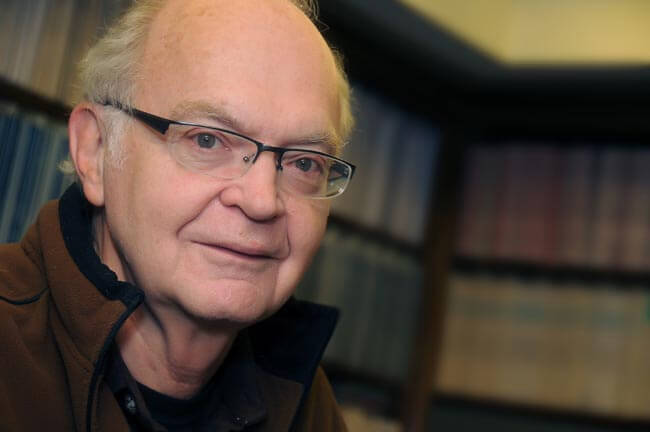
\includegraphics[width=.55\textwidth]{Donald-Knuth.jpg}
\end{center}
    Donald Knuth(Jan. 10, 1938--): Turing Award(1974),
    National Acadamy of Sciences(1975) and many other awards and honors.
\end{frame}

\begin{frame}{What is \LaTeX}
\begin{itemize}
    \item \TeX{} system is too primitive. Leslie Lamport developed a document
    preparation system based on \TeX{} (1984).

    \item \LaTeX{} is short for Lamport TeX{}.
\end{itemize}
\begin{center}
    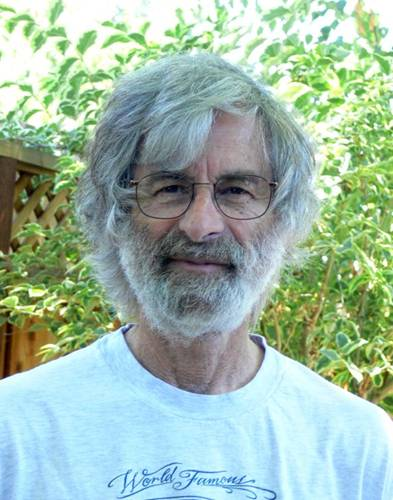
\includegraphics[width=.4\textwidth]{Leslie-Lamport.jpg}
\end{center}
    Leslie Lamport (Feb. 7, 1941--),
    John von Neumann Medal (2008),
    Turing Award(2013), ACM Fellow(2014).
\end{frame}

\begin{frame}{Why use \TeX{} and why not}
\LaTeX{} featues:
\begin{itemize}
    \item Very good at writing structured documents.
    \item Typesetting of complex mathematical formulas.
    \item Control over large documents containing sectioning,
        cross-references, tables and figures.
    \item Contents, footnotes, indexes, ..., become very easy.
    \item Using plain text as opposed to the formatted text, 
        makes the documents readable, small, easy to edit and to compare.
    \item Consistency.
    \item \TeX{} system is free of charge.
\end{itemize}

    But \TeX{} is not always the choice:
\begin{itemize}
    \item Very hard to write unstructured and disorganized documents
        (seminar presentations for example).
    \item Template designing takes a lot of time.
\end{itemize}
\end{frame}

\section{Beginners}
\begin{frame}{\TeX{} source file}
\lstset{language={[LaTeX]TeX}}
\lstinputlisting[keywordstyle=\color{red}]{einstein.tex}
\end{frame}

\begin{frame}{\TeX{} distributions}
\begin{table}
\centering
    \caption{\TeX{} distributions}
    \begin{tabular}{cc}\hline\hline
        OS          &   Distro\\\hline
        All-platform & TeX Live\\
        Windows    & MikTeX \\
        Mac OS    & MacTeX\\\hline
    \end{tabular}
\end{table}

    We write \TeX{} document using text editor, and xelatex to compile
    \TeX{} to produce PDF:
   \\ ~ \\

   \qquad \$ xelatex einstein.tex

\end{frame}

\begin{frame}{Learning curve}
    As my experience, here gives a comparision between 
    \LaTeX{} and Word processors(MS-word, Libre Office, etc.):
\begin{itemize}
    \item 10 minutes of learning ``WORD'', may write a not-so-bad document.
    \item 1 -- 2 hours of learning \LaTeX{} can produce a not-so-bad
        PDF without too complex formulae, figures, and misc., almost
        no publishing mistakes.
    \item About 10 hours of learning \LaTeX{}, you can produce hundreds
        of pages of professional document including contents,
        cross-references, formulae, figures, tables, ...
    \item Few person can write no publishing mistakes in his thesis.doc.
\end{itemize}
\end{frame}

\section{Document Structure}
\begin{frame}{Commands and Environments}
\begin{itemize}
    \item A command starts with backslash and then have a name
        consisting of letters only.
    \item Some commands require parameters. parameters are put in 
        \{\ \ \} after command. Some commands take optional parameters.
        Optional parameter is put in [\ \ ].


        \textbackslash command[optional parameter]\{parameter\}\{parameter\}
\end{itemize}

Environments are special command using \textbackslash begin
    and \textbackslash end

\end{frame}

\begin{frame}{Text}
    \TeX{} use following characters:
\begin{itemize}
    \item Letters, digits and most ASCII chars are used as normal.
    \item Multiple white spaces, tabstops are equal to one white space.
    \item Multiple blank lines are equal to one blank, which produce
        a paragraph separation.
    \item Some special characters must put a prefix backslash:\\
        \#, \%, \^, \&, \_, \{, \}, \~{}
    \item Double backslash is used for line breaking(compare to paragraph).
        \alert{\textbackslash textbackslash} produce one backslash.
\end{itemize}
\end{frame}

\begin{frame}{Sentence and Paragraph}
\begin{itemize}
    \item A group of text between blank lines forms a paragraph.
    \item In English documents, the first paragraph of each section
        is not indented by default.
    \item words which put in a box are not broken by newline. ie.
        \textbackslash mbox\{World-War-III\}.
    \item Command \alert{\textbackslash newline} or
        \alert{\textbackslash newpage} will change the form of a paragraph.
\end{itemize}
\end{frame}

\begin{frame}{Document Structure}
Paragraphs are organized into sections.
A document is structured using following sectioning:
\begin{itemize}
    \item \textbackslash part\{...\}
    \item \textbackslash chapter\{...\} (\alert{not used in article class})
    \item \textbackslash section\{...\}
    \item \textbackslash subsection\{...\}
    \item \textbackslash subsubsection\{...\}
    \item \textbackslash paragraph\{...\}
    \item \textbackslash subparagraph\{...\}
\end{itemize}

Sections are automatically numbered. You should not number chapters
and sections intentionally. Besides, equations, thereoms, figures,
tables, etc. are also numbered automatically.
\end{frame}

\begin{frame}{Big Projects}
    Big document can be split into several parts. \LaTeX{} uses
    command \alert{\textbackslash include} or \alert{\textbackslash input}
    to insert the contents of a file.


\end{frame}

\begin{frame}[fragile]{Lists}
    \LaTeX{} use 3 basic lists: itemize, enumerate and description.

\begin{verbatim}
Fibonacci function:
\begin{enumerate}
    \item BEGIN
    \item if $n<2$ then return 1, goto \ref{end}
    \item calculate fib(n-1) and fib(n-2)
    \item return fib(n-1)+fib(n-2)
    \item END \label{end}
\end{enumerate}
\end{verbatim}

\begin{boxedminipage}{0.8\textwidth}
Fibonacci function:
\begin{enumerate}
    \item BEGIN
    \item if $n<2$ then return 1, goto \ref{end}
    \item calculate fib(n-1) and fib(n-2)
    \item return fib(n-1)+fib(n-2)
    \item END \label{end}
\end{enumerate}
    \end{boxedminipage}
\end{frame}

\section{Math Notation}
\begin{frame}{Math Mode}
    Inline and standalone math notatons look different. Math symbols
    use different font from text.
\begin{itemize}
    \item Inline math mode between \$ and \$: $n!=\prod_{i=0}^n i$
    \item Standalone math mode between \$\$ and \$\$, or in
        \alert{equation} environment. Equation environment will
        automatically numbered.

        \begin{equation}
            \sum_{i=0}^n i = \frac{n (n-1)}{2}
        \end{equation}
        \begin{equation}
            X(\omega) = \int_{-\infty}^{+\infty}
                x(t) e^{-j\omega t}\mathrm{d} t
        \end{equation}
    \item Greek letters: \textbackslash alpha, \textbackslash beta ,...

\end{itemize}
\end{frame}

\begin{frame}{Newtheorem}

{\em Lemmas, Definitions, Axioms} and similar structures are often used
in mathematical documents.
\ \\ \ \\

\qquad \textbackslash newtheorem\{name\}[counter]\{text\}[section]
\ \\ \ \\

\alert{name} is a new environment name. \alert{text} is the text
printed in the document as a label. \alert{counter} specifies the 
name of a previously declared {\em theorem}. \alert{section} specifies
the sectional unit within which the {\em theorem} should get its numbers.

\end{frame}

\section{Figures and Tables}
\begin{frame}[fragile]{Figures and Tables}
    Figures and tables are called floating object, because they occupy
    large space, ie. they may not appear in the current context.
    Therefore, you should avoid using ``See figure below'' or
    ``Refer the table above'' in your documents.

\begin{verbatim}
\begin{figure}
\centering
  \includegraphics[width=0.5\textwidth]{Knuth.jpg}
  \caption{Doland Knuth(1938--)}\label{knuth}
\end{figure}
\end{verbatim}

    \LaTeX{} support both vector graphics(PDF, EPS) and raster grahpics
    (JPG, PNG, BMP, etc.).

\end{frame}

\begin{frame}[fragile]{Figures and Tables}
\begin{verbatim}
\begin{table}
\centering \caption{\TeX{} distributions}
  \begin{tabular}{l|cr}\hline\hline
    OS           & Distro   & Editor\\\hline
    All-platform & TeX Live & \\
    Windows      & MikTeX   & TexMaker\\
    Mac OS       & MacTeX   & TeXShop\\\hline
  \end{tabular}
\end{table}
\end{verbatim}
    \alert{r}, \alert{c} and \alert{l} specify alignment.
    \alert{\&} used as field separation. \alert{$|$} draws vertical
    line, \alert{\textbackslash hline} draws a horizontal line.
\end{frame}

\section{Packages}
\begin{frame}
    \TeX{} distributions come with a large number of packages prein-
    stalled.
\begin{description}
    \item [geometry] Customizing page layout, including papersize,
        margins, etc.
    \item [fancyhdr] Customizing header and footer.
    \item [listings] Printing source codes with syntax highlight.
    \item [hyperref] Creating hyperlink.
    \item [makeidx] Make index.
    \item [longtable] (guess what)
    \item [ctex] CJK (Chinese, Japanese and Korean) language support
    \item [...]
\end{description}
\end{frame}

\section{Cross References}
\begin{frame}{Cross References}
    Almost all tags (using \textbackslash label\{...\})
    can be referenced: figure, table, equation,
    chapter and section, page, etc.
\begin{itemize}
    \item The theory is illustrated in equation
        \alert{\textbackslash ref\{mass-energy\}} in page 
        \alert{\textbackslash pageref\{mass-energy\}} of chapter
        \alert{\textbackslash ref\{einstein\}}.

    \item \textbackslash bibitem in bibliography is cited using
        \textbackslash cite\{\ \ \}.
\end{itemize}
Build bibtex needs 4 steps:
\begin{enumerate}
    \item xelatex foo.tex $\to$ foo.aux, foo.bib
    \item bibtex foo.aux  $\to$ foo.bbl
    \item xelatex foo.tex, insert labels
    \item xelatex foo.tex, correct order
\end{enumerate}
\end{frame}

\begin{frame}{Bibliography}

 Following articles and books are referenced in this text:
    \cite{Knuth_texbook}, \cite{texmanual}, \cite{David_tex_land} and
    \cite{website:top500}.


    \bibliographystyle{unsrt}
    \bibliography{bookref}
\end{frame}
\end{document}
